\chapter{Développement et implémentation}
\label{chap:developpement}

Ce chapitre présente la mise en œuvre concrète du système de prédiction du temps de cuisson des haricots, depuis la préparation des données jusqu’au déploiement embarqué. Il s’appuie sur la méthodologie définie au Chapitre~\ref{chap:methodologie} et reprend strictement les choix techniques (prétraitements, architectures candidates, schéma d’entraînement et optimisation TinyML).

\section{Environnement de développement}
\label{sec:env_dev}

\subsection{Matériel}
Les expérimentations ont été menées sur :
\begin{itemize}
	\item \textbf{Machine locale} : Intel Core i7 (4 cœurs), 16~Go RAM.
	\item \textbf{Google Colab} : session \texttt{Tesla T4} (15~Go VRAM, 12~Go RAM, 118~Go stockage).
	\item \textbf{Samsung Galaxy Note 9} : Octa-core, 6 Go RAM, 128~Go stockage, Android 10.
\end{itemize}

\subsection{Logiciels et versions}
Sauf mention contraire, les versions utilisées sont celles définies en méthodologie :
\begin{itemize}
	\item \textbf{Python} 3.10
	\item \textbf{TensorFlow} 2.19 pour l'entrainement et \textbf{TensorFlow} 2.13 pour la quantification \& API Keras (compatibles \texttt{TensorFlow Lite})
	\item \textbf{Pandas} 2.1, \textbf{NumPy} 1.25, \textbf{Matplotlib} 3.8
\end{itemize}

\section{Préparation des données}
\label{sec:pretraitement}

Le protocole de préparation suit \textit{strictement} le Chapitre~\ref{chap:methodologie} :
\begin{enumerate}
	\item \textbf{Recadrage centré} et \textbf{redimensionnement} des images brutes (\(3000\times4000\)) en \(224\times224\).
	\item \textbf{Mise à l’échelle} des pixels dans \([0,1]\).
	\item \textbf{Augmentation} stochastique \textit{train-only} (flips, crops, jitter de luminosité/contraste/saturation, blur, bruit gaussien)\footnote{Paramètres détaillés : voir Chap.~\ref{chap:methodologie}.}.
	\item \textbf{Normalisation Min--Max} des labels \(T_c\in[0,1]\), calculée uniquement sur \(\mathcal{D}_{\text{train}}\), appliquée à val/test, puis inversée pour restituer les minutes en sortie.
	\item \textbf{Export HDF5} par split avec clés \texttt{images}, \texttt{cooking\_times}.
\end{enumerate}

%%%%%%%%%%% Pré-entrainement %%%%%%%%%%%%%%%%%%%%%%%%%%%%%%%%%%%%%%%%%

\begin{verbatim}
\small
1. Charger le fichier CSV contenant les chemins d’images et les étiquettes (labels).
2. Extraire la liste des chemins d’images et convertir les labels au format float.
3. Définir les transformations de base (redimensionnement, conversion en tenseur).
4. Définir les transformations d’augmentation de données 
   (redimensionnement, recadrage aléatoire, flips, jitter couleur, flou gaussien).
5. Pour chaque chemin d’image :
    a. Ouvrir l’image et la convertir en RGB.
    b. Appliquer la transformation de base.
    c. Convertir l’image en tableau numpy uint8 et l’ajouter à la liste des images de base.
6. Convertir la liste des images et labels en tableaux numpy.
7. Normaliser les labels entre 0 et 1.
8. Séparer le jeu de données en ensembles d'entraînement, de validation et de test 
   (stratification sur les labels).
9. Pour chaque image de l’ensemble d’entraînement :
    a. Ajouter l’image originale et son label.
    b. Pour un nombre donné d’augmentations :
        i. Convertir l’image en format PIL.
       ii. Appliquer les transformations d’augmentation.
      iii. Convertir l’image augmentée au format numpy uint8.
       iv. Ajouter l’image augmentée et le label à la liste.
10. Convertir les listes d’images et labels augmentés en tableaux numpy.
11. Enregistrer chaque ensemble (entraînement, validation, test) dans un fichier HDF5, 
    avec deux jeux de données : images et labels (temps de cuisson).
\end{verbatim}

\section{Architectures de modèles}
\label{sec:modeles}

Conformément à la méthodologie :
\begin{itemize}
	\item \textbf{CNN personnalisés} (deux variantes) pour une extraction hiérarchique efficace.
	\item \textbf{MobileNetV2}, \textbf{EfficientNetB0}, \textbf{NASNetMobile} (apprentissage par transfert).
\end{itemize}

La tête de régression est composée d’une couche de sortie scalaire (\texttt{linear}).
La régularisation inclut un \texttt{dropout} de 0.3 et une pénalisation L2 (\(\lambda=10^{-4}\)).

%%%%%%%%%%% Tableau des hyperparamètres %%%%%%%%%%%%%%%%%%%%%%%%%%%%%%%%%%%%%%%%%
\begin{table}[h!]
	\centering
	\caption{Hyperparamètres d’entraînement retenus.}
	\label{tab:hyperparams}
	\begin{tabular}{l l}
		\toprule
		Paramètre                    & Valeur                                             \\ \midrule
		Optimiseur                   & Adam (\(\beta_1=0.9\), \(\beta_2=0.999\))          \\
		Taux d’apprentissage initial & \(10^{-4}\) + scheduler \texttt{ReduceLROnPlateau} \\
		Fonction de perte            & MSE                                                \\
		Métriques                    & MAE, RMSE, \(R^2\)                                 \\
		Batch size                   & 32                                                 \\
		Époques max                  & 100                                                \\
		Patience early stopping      & 5                                                  \\
		Dropout                      & 0.3                                                \\
		Régularisation L2            & \(10^{-4}\)                                        \\ \bottomrule
	\end{tabular}
\end{table}

\section{Stratégie d’entraînement}
\label{sec:entrainement}

Le modèle est entraîné sur \(\mathcal{D}_{\text{train}}\), validé sur \(\mathcal{D}_{\text{val}}\).
L’\textit{early stopping} permet d’éviter le surapprentissage.

%%%%%%%%%%%%%%%%%%%%%%%%%%%%%%% Fonction d'entrainement des modèles %%%%%%%%%%%%%%%%%%%%%%%%%%%%%%%
\begin{verbatim}
\small
1. Initialiser les variables pour la meilleure validation MAE et le compteur de patience.
2. Construire une nouvelle instance du modèle via la fonction model_builder.
3. Initialiser un dictionnaire pour stocker l’historique d’entraînement.
4. Charger le jeu de données d’entraînement à partir du chemin donné.
5. Calculer le nombre d’itérations (steps) par époque selon la taille du batch.
6. Pour chaque époque dans le nombre total d’époques :
    a. Afficher l’information de l’époque en cours.
    b. Créer un générateur de batchs d’entraînement.
    c. Entraîner le modèle sur une époque complète avec le générateur.
    d. Récupérer la perte (loss) et la MAE d’entraînement.
    e. Évaluer le modèle sur les données de validation pour obtenir val_loss et val_mae.
    f. Enregistrer ces métriques dans l’historique.
    g. Afficher un résumé des résultats d’entraînement et de validation.
    h. Appliquer une stratégie d’early stopping :
        i. Si val_mae s’améliore, sauvegarder le modèle et réinitialiser le compteur de patience.
       ii. Sinon, incrémenter le compteur de patience.
      iii. Si le compteur atteint la patience maximale, arrêter l’entraînement prématurément.
    i. Libérer la mémoire du générateur.
7. Afficher la fin de l’entraînement.
8. Fermer le loader de données.
9. Retourner l’historique d’entraînement.
\end{verbatim}

\section{Export et optimisation TinyML}
\label{sec:optim_tinyml}

\subsection{Conversion TensorFlow Lite (float16)}
La quantification retenue est \textbf{float16}, permettant de réduire la taille mémoire d’environ 50\% tout en préservant la précision.

%%%%%%%%%%%%%%%%%%%% Conversion du modèle %%%%%%%%%%%%%%%%%%%%%%%%%%%%%%%%%%%%%%%%
\begin{verbatim}
1. Importer la bibliothèque TensorFlow (version 2.13).
2. Charger le modèle enregistré (SavedModel).
3. Initialiser un convertisseur TFLite à partir du modèle chargé.
4. Activer les optimisations par défaut pour la conversion.
5. Spécifier que le type de données cible est float16 (pour Android).
6. Convertir le modèle en format TFLite.
7. Sauvegarder le modèle TFLite dans un fichier binaire.
8. Afficher un message de succès de la conversion.
\end{verbatim}

\section{Déploiement Android}
\label{sec:deploiement_android}

\subsection{Cible et outils}
\begin{itemize}
	\item \textbf{Android Studio} Narwhal (2025.1.2), \textbf{SDK} Android 36.
	\item Compatibilité descendante : \texttt{minSdkVersion=26} (Android 8.0).
	\item \textbf{Langage} : Kotlin.
	\item \textbf{Runtime ML} : \texttt{TensorFlow Lite Interpreter} v2.13.
\end{itemize}

\subsection{Intégration et inférence}
Le modèle \texttt{.tflite} est placé dans \texttt{assets/}.
Le pipeline embarqué applique le même prétraitement (resize \(224\times224\), normalisation), puis l’inférence, suivie de l’inversion Min--Max pour obtenir le temps en minutes.

%%%%%%%%%%%%%%%%%%%%% Deploiement sur Android %%%%%%%%%%%%%%%%%%%%%%%%%%%%%%
\begin{verbatim}
\small
1. MainViewModel (ViewModel) :
    - Définir états observables : imageBitmap, predictionResult.
    - Constantes : taille image (224x224), min/max temps cuisson.
    - loadModelFile(context, modelPath) : charger modèle TFLite depuis assets.
    - runPrediction(context, bitmap) :
        a. Mettre à jour imageBitmap et predictionResult.
        b. Lancer coroutine pour exécuter runModelInference.
        c. Mesurer latence et mettre à jour predictionResult.
        d. Gérer erreurs.
    - runModelInference(context, bitmap) :
        a. Convertir bitmap en ARGB_8888 si nécessaire.
        b. Redimensionner à 224x224.
        c. Créer ByteBuffer, normaliser pixels [0,1].
        d. Charger interpréteur TFLite.
        e. Exécuter inférence et récupérer sortie.
        f. Dénormaliser prédiction et retourner.
    - denormalize(normalizedValue) : convertir sortie normalisée en valeur réelle.
    - reset() : réinitialiser états.
2. IntroManager :
    - Gérer SharedPreferences pour écran d’introduction.
    - shouldShowIntro() : retourner booléen.
    - setShowIntro(shouldShow) : modifier préférence.
3. MainActivity :
    - Initialiser IntroManager.
    - Afficher IntroScreen si besoin, sinon écran prédiction.
    - Navigation entre PredictionScreen et InfoScreen.
4. Composables UI :
    - IntroScreen : boîte de dialogue avec option "ne plus afficher".
    - PredictionScreen :
        a. Gérer permissions caméra, sélection image galerie/camera.
        b. Afficher image sélectionnée.
        c. Afficher résultats prédiction (temps, RMSE, MAE).
        d. Boutons importer, prendre photo, réinitialiser.
    - InfoScreen :
        a. Présentation app.
        b. Explication métriques MAE et RMSE.
        c. Contexte cuisson haricots.
\end{verbatim}

\paragraph{UI/Workflow.}
\begin{figure}[H]
	\centering
	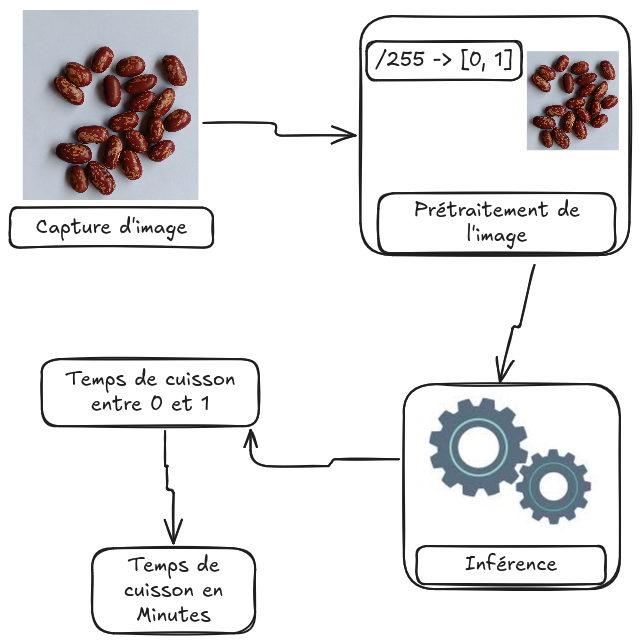
\includegraphics[width=0.9\textwidth]{figures/workflow.png}
	\caption{Workflow fonctionnel de l’application Android : capture ou import d’image, prétraitement, inférence et affichage du temps de cuisson (\(T_c\)).}
	\label{fig:app_workflow}
\end{figure}

\section{Mesures et artefacts à produire}
\label{sec:mesures_artefacts}

Cette section ne présente \emph{pas} de résultats chiffrés (qui seront rapportés au Chapitre Résultats), mais liste les artefacts générés.

\begin{table}[h!]
	\centering
	\caption{(Placeholder) Synthèse des modèles déployables.}
	\label{tab:deploy_synthese}
	\begin{tabular}{@{}lcccc@{}}
		\toprule
		Modèle         & Fichier TFLite     & Taille (Mo) & Latence (ms)\textsuperscript{$\dagger$} & Notes   \\ \midrule
		TBNet2         & model\_fp16.tflite & 0.9         & 187                                     & float16 \\
		MobileNetV2    & model\_fp16.tflite & 7.2         & 734                                     & float16 \\
		EfficientNetB0 & model\_fp16.tflite & 8.7         & 769                                     & float16 \\
		NASNetMobile   & model\_fp16.tflite & 21.3        & 867                                     & float16 \\ \bottomrule
	\end{tabular}
\end{table}

\footnotesize{$\dagger$ Mesures effectuées sur appareil cible (moyenne et percentiles).}

\section{Limites pratiques et points d’attention}
\label{sec:limites}
\begin{itemize}
	\item \textbf{Alignement des prétraitements} : le pipeline embarqué doit reproduire fidèlement la normalisation et l’inversion Min--Max.
	\item \textbf{Latence et consommation} : fortement dépendantes de l’appareil et des délégués (CPU/GPU/NNAPI).
	\item \textbf{Gestion mémoire} : réutilisation des buffers d’E/S et chargement paresseux recommandés côté Android.
	\item \textbf{Robustesse applicative} : prévoir la gestion des erreurs (fichier image invalide, absence d’entrée).
\end{itemize}

\bigskip
\noindent \textbf{Résumé} — Ce chapitre documente l’implémentation complète (prétraitement, modèles, entraînement, conversion float16, intégration Android) et définit les artefacts à produire. Les résultats expérimentaux seront présentés et analysés au Chapitre~\ref{chap:resultats_discussion}.
